% !TEX root = Projektdokumentation.tex
\section{Beispiel 3}
\label{sec:beispiel3}

\subsection{Ausgangssituation} 
\label{sec:ausgangssituation3}
In Abschnitt \ref{sec:voraussetzungen} wurde beschrieben, dass die Schulze Methode auch Ergebnisse liefert, wenn Kandidaten gleich oder nicht bewertet wurden. Nicht bewertete Kandidaten werden dabei behandelt, als wären sie alle vom Wähler auf dem letzten Platz gewählt worden, sodass jeder Kandidat, der vom Wähler bewertet wurde, den nicht bewerteten Kandidaten vorgezogen wird. Diese Beispiel bezieht sich auf das sechste Beispiel von \glqq A New Monotonic, Clone-Independent,
Reversal Symmetric, and Condorcet-Consistent
Single-Winner Election Method \grqq{}\footnote{\Vgl \citet{Schulze2017} Kapitel 3.6}.

\begin{description}
\centering
\item[6 mal] $a \succ_{v} b \succ_{v} c \succ_{v}d$
\item[8 mal] $a \approx_{v} b \succ_{v} c \approx_{v}d$
\item[8 mal] $a \approx_{v} c \succ_{v} b \approx_{v}d$
\item[18 mal] $a \approx_{v} c \succ_{v} d \succ_{v}b$
\item[8 mal] $a \approx_{v} c \approx_{v} d \succ_{v}d$
\item[40 mal] $b \succ_{v} a \approx_{v} c \approx_{v}d$
\item[4 mal] $c \succ_{v} b \succ_{v} d \succ_{v}a$
\item[9 mal] $c \succ_{v} d \succ_{v} a \succ_{v}b$
\item[8 mal] $c \approx_{v} d \succ_{v} a \approx_{v}b$
\item[14 mal] $d \succ_{v} a \succ_{v} b \succ_{v}c$
\item[11 mal] $d \succ_{v} b \succ_{v} c \succ_{v}a$
\item[4 mal] $d \succ_{v} c \succ_{v} a \succ_{v}b$
\end{description}

Zur Erläuterung wird die Wahl $a \approx_{v} b \succ_{v} c \approx_{v}d$ betrachtet. Hier hat der Wähler gesagt, er möchte lieber Kandidat $a$ oder $b$ haben, welcher ist ihm dabei gleich, aber lieber einen von den beiden Kandidaten, als die Kandidaten $c$ oder $d$. Dort macht der Wähler aber auch kein Unterschied ob $c$ oder $d$, beide findet er gleich gut/schlecht.

\subsection{Lösungsschritte} 
\label{sec:loesungen3}
Als erstes muss die Menge $N$ bestimmen werden, in der man die Kandidaten gegeneinander antreten lässt, nur kann es diesmal zu Duellen ohne Sieger kommen, da beide Kandidaten gleich bewertet wurden. Diese Stimmen werden dann nicht Berücksichtigt. 

Exemplarisch wird in Tabelle \ref{beispiel3ab} das Duell von Kandidat $a$ gegen Kandidat $b$ dargestellt. 

% !TEX root = Projektdokumentation.tex

\begin{longtable}[c]{|l|l|l|l|}
\hline
Duelle & $a$  & $b$  & Sieger \\ \hline
\endfirsthead
%
\endhead
%
1      & 6  &    & $a$      \\ \hline
\rowcolor[HTML]{9B9B9B} 
2      & 8  & 8  & keiner \\ \hline
3      & 8  &    & $a$      \\ \hline
4      & 18 &    & $a$     \\ \hline
5      & 8  &    & $a$    \\ \hline
6      &    & 40 & $b$    \\ \hline
7      &    & 4  & $b$     \\ \hline
8      & 9  &    & $a$    \\ \hline
\rowcolor[HTML]{9B9B9B} 
9      & 8  & 8  & keiner \\ \hline
10     & 14 &    & $a$    \\ \hline
11     &    & 11 & $b$    \\ \hline
12     & 4  &    & $a$    \\ \hline
Summe  & 67 & 55 &        \\ \hline
\caption{Duell $a$ gegen $b$, graue Felder sind nicht bewertet, da unentschieden (Beispiel 3)}
\label{beispiel3ab}\\
\end{longtable}


Wenn man dieses Verfahren für alle Kandidaten anwendet erhält man die Menge $N$, die in Tabelle \ref{beispiel3N} aufgetragen ist.

% !TEX root = Projektdokumentation.tex

\begin{longtable}[c]{|l|l|l|l|l|}
\hline
            & N{[}*,a{]} & N{[}*,b{]} & N{[}*,c{]} & N{[}*,d{]} \\ \hline
\endfirsthead
%
\endhead
%
N{[}a, *{]} & ---        & 67         & 28         & 40         \\ \hline
N{[}b, *{]} & 55         & ---        & 79         & 58         \\ \hline
N{[}c, *{]} & 36         & 59         & ---        & 45         \\ \hline
N{[}d, *{]} & 50         & 72         & 29         & ---        \\ \hline
\caption{Die Menge $N$ (Beispiel 3)}
\label{beispiel3N}\\
\end{longtable}

In Abbildung \ref{fig:graph3} sieht man den Graphen, der aus der Menge $N$ gebildet wurde, er sieht etwas anders aus als in Beispiel 1 und Beispiel 2, da der Wert für den Weg von Kandidat $a$ nach Kandidat $b$, sondern auch den umgekehrten Weg von $b$ nach $a$ benötigt wird, sprich es werden die Stimmen für den Kandidaten $a$ und die Gegenstimmen eingezeichnet. 

\begin{figure}[!h]
\centering
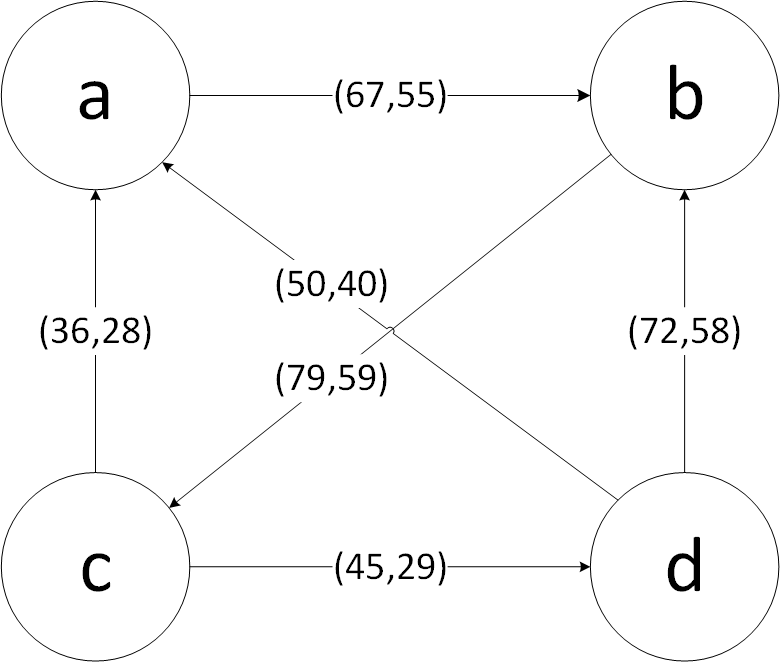
\includegraphics[scale=0.5]{Bilder/Beispiel3_Graph.png}
\caption{Graph über die Menge $N$(Beispiel 3)}
\label{fig:graph3}
\end{figure}

Es gibt verschiedene Möglichkeiten einen Gewinner mit der \schulze zu finden, da es verschiedene  Ansätze gibt die stärke eines Weges zu bestimmen. Die Methoden die in diesem Abschnitt vorgestellt werden sind margin, ratio, winning votes und losing votes.  Wenn alle Wähler die Kandidaten in eine strikte Ordnung gebracht haben, wie in den Beispielen 1 und 2, dann geben diese Methoden immer das selbe Ergebnis, wenn

\begin{align*}
& \forall (x_{1},x_{2}),(y_{1},y_{2}) \in \mathbb{N}_0 	\times \mathbb{N}_0 \\
((x_{1} > y_{1} \textrm{ und }  x_{2}\leq y_{2}) & \textrm{ oder } (x_{1} \geq y_{1} \textrm{ und } x_{2} < y_{2}))\Rightarrow (x_{1},x_{2}) \succ_{D} (y_{1},y_{2})
\end{align*}

gilt. Dies gilt für die vier Methoden die Vorgestellt werden, da dort die Stimmen für den Kandidaten zusammen mit den Gegenstimmen immer der Anzahl der Wähler, also $C$ ergibt und wenn die eine Verbindung mehr Stimmen für den Kandidaten hat ($x_{1} > y_{1}$) muss daraus folgen, dass die Verbindung $y$ mehr Gegenstimmen ($y_{2}$) hat als die Verbindung $x$. $(x_{1},x_{2})$, $(y_{1},y_{2})$ sind dabei Verbindungen zweier Kandidaten in der vollständigen Schreibweise, die als zweiten Wert die Gegenstimmen enthält, Abschnitt \ref{sec:verbindung}. Da alle vier Methoden der Definition entsprechen, ist es auch legitim, dass die Beispiele 1 und 2 mit der winning votes Methode arbeiten und die verkürzte Schreibweise genutzt haben, genauso könnten die anderen drei Methoden eingesetzt werden.

Wenn die Wähler nicht alle Kandidaten in eine strikte Reihenfolge bringen und Kandidaten gleich bewerten, geben diese Methoden je nach Situation gleiche oder unterschiedliche Ergebnisse aus, da die obige Definition nicht mehr passt, da nun Stimmen für den Kandidaten zusammen mit den Stimmen gegen den Kandidaten nicht der Anzahl der Wähler ($C$) entsprechen muss.
Dieses Beispiel ist so aufgebaut, dass jede Methode einen anderen Kandidaten als Sieger ausgibt. Daher ist es wichtig vor der Wahl zu definieren, welche Wahlmethode genutzt wird.

\subsubsection{margin}
\label{sec:margin}
Beim Ansatz $margin$ gewinnt der Kandidat, der seinen Sieg mit einem größeren Abstand erreicht. 
Untersucht wir Beispielhaft das Duell $a$ gegen $b$. Der Stärkste Weg von $a$ nach $b$, ist die direkt Verbindung, Kandidat $a$ erhält 67 Stimmen und Kandidat $b$ nur 55 Stimmen und damit gewinnt Kandidat $a$ mit 12 Stimmen Vorsprung. 
Aber auch Kandidat $b$ kann Kandidat $a$ schlagen, der Stärkste Weg für dieses Duell ist von $b$ über $c$ und $d$ nach $a$. Die schwächste Verbindung in diesem Weg ist die Verbindung $d$ nach $a$, da dort mit nur 10 Stimmen Vorsprung der Kandidat $d$, Kandidat $a$ schlägt.
Um den Gewinner festzustellen wird der Abstand für den Sieg von $a$ (12 Stimmen) mit dem Sieg von $b$ (10 Stimmen) verglichen und der Gewinner dieses Duells ist $a$, mit zwei Stimmen Vorsprung.

Auch hier wurde in Tabelle \ref{beispiel3margin_p} die Menge $P$ aufgestellt. Die Werte in der Tabelle zeigen nun den Abstand, mit dem der Kandidat den Gegner geschlagen hat.

% !TEX root = ../Projektdokumentation.tex
\begin{longtable}[c]{|l|l|l|l|l|}
\hline
            & P{[}*,a{]} & P{[}*,b{]} & P{[}*,c{]} & P{[}*,d{]} \\ \hline
\endfirsthead
%
\endhead
%
P{[}a, *{]} & ---        & 12         & 12         & 12         \\ \hline
P{[}b, *{]} & 10         & ---        & 20         & 16         \\ \hline
P{[}c, *{]} & 10         & 14         & ---        & 16         \\ \hline
P{[}d, *{]} & 10         & 14         & 14         & ---        \\ \hline
\caption{Die Menge $P$ nach margin Regel(Beispiel 3)}
\label{beispiel3margin_p}\\
\end{longtable}

Anschließend wird mit den Werten der Menge $P$ die neu Zweikampfsituation erstellt und man erhält die Relation $\mathcal{O}_{margin} = \{ ab, ac,ad,bc,bd,cd \}$

Daraus ergibt sich die Ergebnismenge $\mathcal{S}_{margin} \in \{ a\}$ und der Sieger unter Berücksichtigung des Abstandes ist Kandidat $a$.

\subsubsection{ratio}
\label{sec:ratio}
Eine weitere Methode die eingesetzt wird, um einen Sieger zu erhalten ist ein Verhältnis (eng: ratio) zu ermitteln. Hierzu werden die Stimmen für den Sieger durch die Stimmen gegen den Sieger geteilt und damit das Verhältnis ausgerechnet, mit dem der Sieger gewonnen hat.

Beispielhaft wird wieder das Duelle von Kandidat $a$ gegen Kandidat $b$ betrachtet. Im Duell $a$ gegen $b$ ist, wie im Vergleich über den Abstand (Abschnitt \ref{sec:margin}), der direkte Weg der stärkste Weg. Der Stärkste Weg von Kandidat $b$ zu Kandidat $a$ ist im Vergleich über das Verhältnis aber ein anderer. Er führt von $b$ über $c$ nach $a$ . Die kritische Verbindung ist in diesem Fall die Verbindung von $c$ nach $a$, da hier ein Verhältnis von $36/28 \approx 1,286$, das kleinste Verhältnis auf diesem Weg darstellt. Wird der Weg von Kandidat $b$ nach $a$ aus Abschnitt \ref{sec:margin} untersucht, ist dort die Kritische Verbindung $d$ nach $a$, was ein Verhältnis von $ 50/40 = 1,25$ darstellt und damit eine schlechteres Verhältnis als der Weg $b$ über $c$ nach $a$ hat.

Die Berechnung der besten Verhältnisse wird wieder für alle Duelle gemacht und  Tabelle \ref{beispiel3ratio_p} zeigt die Menge $P$ unter Betrachtung des Verhältnisse.

% !TEX root = ../Projektdokumentation.tex
\begin{longtable}[c]{|l|l|l|l|l|}
\hline
            & P{[}*,a{]} & P{[}*,b{]} & P{[}*,c{]} & P{[}*,d{]} \\ \hline
\endfirsthead
%
\endhead
%
P{[}a, *{]} & ---        & 1,218      & 1,218      & 1,218      \\ \hline
P{[}b, *{]} & 1,286      & ---        & 1,339      & 1,339      \\ \hline
P{[}c, *{]} & 1,286      & 1,241      & ---        & 1,552      \\ \hline
P{[}d, *{]} & 1,25       & 1,241      & 1,241      & ---        \\ \hline
\caption{Die Menge $P$ nach ratio Regel(Beispiel 3)}
\label{beispiel3ratio_p}\\
\end{longtable}

Anschließend wird mit den Werten der Menge $P$ die neu Zweikampfsituation erstellt und man erhält die Relation $\mathcal{O}_{ratio} = \{ ba,bc,bd,ca,cd,da \}$

Daraus ergibt sich die Ergebnismenge $\mathcal{S}_{ratio} \in \{ b\}$ und er Sieger unter Berücksichtigung des Verhältnis ist Kandidat $b$.

\subsubsection{winning votes}
\label{sec:winningVotes}
Es kann der Sieger aber auch als die Person gelten, die am meisten Siege hat (eng: winning votes). Dies ist auch das Verfahren, welches in den Beispiel 1 (Abschnitt: \ref{sec:beispiel1}) und Beispiel 2 (Abschnitt: \ref{sec:beispiel2}) eingesetzt wurde. Hier wird untersucht, welcher der beiden Kandidaten gewinnt. Exemplarisch tritt wieder Kandidat $a$ gegen Kandidat $b$ an. Kandidat $a$ schlägt Kandidat $b$ mit der direkten Verbindung mit 67 Stimmen, Kandidat $b$ kann Kandidat $a$ über den Weg $b$ über $c$ und $d$ nach $a$ schlagen. Jedoch ist hier die schwächste Verbindung, die Verbindung $c$ nach $d$ mit nur 45 Stimmen. Diese Werte (Kandidat $a$: 67 Stimmen, Kandidat $b$: 45 Stimmen) werden verglichen und Kandidat $a$ gewinnt. 

Diese Untersuchung wird für alle Duelle gemacht und es ergibt sich die in Tabelle \ref{beispiel3win_p} dargestellte Menge $P$.

% !TEX root = ../Projektdokumentation.tex
\begin{longtable}[c]{|l|l|l|l|l|}
\hline
            & P{[}*,a{]} & P{[}*,b{]} & P{[}*,c{]} & P{[}*,d{]} \\ \hline
\endfirsthead
%
\endhead
%
P{[}a, *{]} & ---        & 67         & 76         & 45         \\ \hline
P{[}b, *{]} & 45         & ---        & 79         & 45         \\ \hline
P{[}c, *{]} & 45         & 45         & ---        & 45         \\ \hline
P{[}d, *{]} & 50         & 72         & 72         & ---        \\ \hline
\caption{Die Menge $P$ nach winning votes Regel(Beispiel 3)}
\label{beispiel3win_p}\\
\end{longtable}


Anschließend wird mit den Werten der Menge $P$ die neu Zweikampfsituation erstellt und man erhält die Relation $\mathcal{O}_{win} = \{ ab,ac,bc,da,db,dc \}$

Daraus ergibt sich die Ergebnismenge $\mathcal{S}_{win} \in \{d\}$ und er Sieger unter Berücksichtigung des Verhältnis ist Kandidat $d$.


\subsubsection{losing votes}
\label{sec:lose}
Ein anderer Ansatz der angewendet werden kann, ist den Kandidaten zum Sieger zu küren, der am wenigsten Gegenstimmen hat (eng. losing votes). Die kritische Verbindung ist dabei die Verbindung, bei der es die meisten Gegenstimmen gibt. Der stärkste Weg ist dann der Weg, bei dem die kritische Verbindung die wenigsten Gegenstimmen hat.

Für dieses Verfahren wird beispielhaft das Duell von Kandidat $a$ und Kandidat $c$ untersucht. Kandidat $a$ kann Kandidat $c$ schlagen über den Weg $a$ über $b$ nach $c$. Dort ist die kritische Verbindung zwischen Kandidat $b$ und $c$, da es an dieser Stelle 59 Gegenstimmen gibt. 
Kandidat $c$ kann Kandidat $a$ über den direkten Weg schlagen und hat dabei nur 28 Gegenstimmen. Die zweite Möglichkeit wäre der Weg von $c$ über $d$ nach $a$, dort wäre die kritische Verbindung von Kandidat $d$ nach $a$ mit 40 Gegenstimmen. Daher wird die Direktverbindung genutzt mit nur 28 Gegenstimmen.
Beide Wege werden nun verglichen und Kandidat $c$ gewinnt gegen Kandidat $a$, da $c$ nur 28 Gegenstimmen hat und Kandidat $a$ 59 Gegenstimmen.

Alle Duelle werde so untersucht, die Ergebnisse, die die Menge $P$ bilden, sind in Tabelle \ref{beispiel3losing_p} eingetragen.

% !TEX root = ../Projektdokumentation.tex
\begin{longtable}[c]{|l|l|l|l|l|}
\hline
            & P{[}*,a{]} & P{[}*,b{]} & P{[}*,c{]} & P{[}*,d{]} \\ \hline
\endfirsthead
%
\endhead
%
P{[}a, *{]} & ---        & 55         & 59         & 59         \\ \hline
P{[}b, *{]} & 59         & ---        & 59         & 59         \\ \hline
P{[}c, *{]} & 28         & 55         & ---        & 29         \\ \hline
P{[}d, *{]} & 40         & 55         & 59         & ---        \\ \hline
\caption{Die Menge $P$ nach losing votes Regel(Beispiel 3)}
\label{beispiel3losing_p}\\
\end{longtable}


Anschließend wird mit den Werten der Menge $P$ die neu Zweikampfsituation erstellt und man erhält die Relation $\mathcal{O}_{los} = \{ ab,ca,cb,cd,da,db \}$

Daraus ergibt sich die Ergebnismenge $\mathcal{S}_{los} \in \{c\}$ und er Sieger unter Berücksichtigung des Verhältnis ist Kandidat $d$.

\subsection{Ergebnis} 
\label{sec:ergebnis3}
Dieses Beispiel zeigt, dass es schwer sein kann zu bestimmen, wann ein Kandidat einen anderen schlägt. Jede Methode ist logisch, korrekt und nachvollziehbar. Das die vier vorgestellten Methoden unterschiedliche Ergebnisse liefern, ist aber nur dann der Fall, wenn es dem Wählern erlaubt ist Kandidaten auch gleich zu bewerten. Daher muss beachtet werden, dass wenn man Kandidaten gleich bewerten kann, vorher festgelegt werden muss, nach welcher Methode die Stimmen bewertet werden, da es sonst unter Umständen zu verschiedenen Siegern kommen kann. Dieses Beispiel wurde extra so von Herrn Schulze in seiner Ausarbeitung \glqq A New Monotonic, Clone-Independent,
Reversal Symmetric, and Condorcet-Consistent
Single-Winner Election Method\grqq{}\footnote{\Vgl \citet{Schulze2017}} konstruiert, dass bei jeder der Methoden unter Abschnitt \ref{sec:loesungen3} immer ein anderer Sieger als Ergebnis geliefert wird. In der Realität kann es auch vorkommen, dass mehrere der vorgestellten Methoden die selben Sieger liefern, auch wenn Kandidaten gleich bewertet wurden.
\newpage